\documentclass[10pt]{article}

\usepackage[T1]{fontenc}
\usepackage{geometry}
\usepackage{amsmath, amssymb, amsthm}
\usepackage{tikz}

\title{Mathematics I - Problem Sheet II}
\author{Satvik Saha}
\date{}

\geometry{a4paper, margin=1in}
\setlength\parindent{0pt}
\renewcommand{\labelenumi}{(\roman{enumi})}
% \renewcommand\qedsymbol{$\blacksquare$}

\begin{document}
        \par\textbf{IISER Kolkata} \hfill \textbf{Problem Sheet II}
        \vspace{3pt}
        \hrule
        \vspace{3pt}
        \begin{center}
                \LARGE{\textbf{MA 1101 : Mathematics I}}
        \end{center}
        \vspace{3pt}
        \hrule
        \vspace{3pt}
        Satvik Saha, \texttt{19MS154}\hfill\today
        \vspace{20pt}

        \textbf{Solution 1.}\\
        Let $R$ be a relation on $\mathbb{R}^2$ such that
        \[(x_1, x_2)\,R\,(y_1, y_2) \quad\text{if}\quad x_1 = y_1.\]
        \begin{enumerate}
                \item For an arbitrary $(x, y)\in\mathbb{R}^2$, $(x, y)\,R\,(x, y)$, since $x = x$. Therefore, $R$ is reflexive.

                For $(x_1, x_2), (y_1, y_2) \in \mathbb{R}^2$, if $(x_1, x_2)\,R\,(y_1, y_2)$, we can write $x_1 = y_1 \Rightarrow y_1 = x_1$.
                Thus, we have $(y_1, y_2)\,R\,(x_1, x_2)$. Therefore, $R$ is symmetric.

                For $(x_1, x_2), (y_1, y_2), (z_1, z_2) \in \mathbb{R}^2$, if $(x_1, x_2)\,R\,(y_1, y_2)$ and $(y_1, y_2)\,R\,(z_1, z_2)$,
                we can write $x_1 = y_1$ and $y_1 = z_1$, from which we have $x_1 = z_1 \Rightarrow (x_1, x_2)\,R\,(z_1, z_2)$.
                Therefore, $R$ is transitive.

                Hence, $R$ is an equivalence relation.\qed

                \item For $(x_1, x_2) \in \mathbb{R}^2$, we have
                \begin{align*}
                [(x_1, x_2)] \;&=\; \{(y_1, y_2) \in \mathbb{R}^2 : (x_1, x_2)\,R\,(y_1, y_2)\} \\
                        \;&=\; \{(y_1, y_2) \in \mathbb{R}^2 : x_1 = y_1\}\\
                        \;&=\; \{(x_1, y) : y \in \mathbb{R}\}
                \end{align*}
                Therefore, the quotient set of $R$ is given by $$\mathbb{R}/R \;=\; \{L_x : x \in \mathbb{R}\},$$
                where $L_x = \{(x, y) : y \in \mathbb{R}\}$.
                Clearly, each equivalence class $L_x \in \mathbb{R}/R$ is a vertical line in the Cartesian plane, passing through $(x, 0)$.\\

                \begin{center}
                \begin{tikzpicture}[scale=1, transform shape]
                        \draw[latex-latex, thick] (0, 5) node[below left]{$y$} -- (0, -5);
                        \draw[latex-latex, thick] (5, 0) node[below left]{$x$} -- (-5, 0);
                        \node[below left] at (0, 0){$O$};
                        \node[below left] at (1, 0){$1$};
                        \node[below left] at (2.71828, 0){$e$};
                        \node[below left] at (-1.414, 0){$-\sqrt{2}$};
                        \draw[<->, color=blue] (1, 5) node[below right]{$L_1$} -- (1, -5);
                        \draw[<->, color=red] (2.71828, 5) node[below right]{$L_e$} -- (2.71828, -5);
                        \draw[<->, color=olive] (-1.414, 5) node[below right]{$L_{-\sqrt{2}}$} -- (-1.414, -5);
                \end{tikzpicture}
                \end{center}
        \end{enumerate}
        \clearpage

        \textbf{Solution 2.}\\
        Let $R$ be a relation on $\mathbb{R}^2$ such that
        \[(x_1, x_2)\,R\,(y_1, y_2) \quad\text{if}\quad x_1^2 + x_2^2 = y_1^2 + y_2^2\]
        \begin{enumerate}
                \item For an arbitrary $(x, y) \in \mathbb{R}^2$, $(x, y)\,R\,(x, y)$, since $x^2 + y^2 = x^2 + y^2$. Therefore, $R$
                is reflexive.

                For $(x_1, x_2), (y_1, y_2) \in \mathbb{R}^2$, if $(x_1, x_2)\,R\,(y_1, y_2)$, we can write 
                $x_1^2 + x_2^2 = y_1^2 + y_2^2 \Rightarrow y_1^2 + y_2^2 = x_1^2 + x_2^2$. Thus, we have $(y_1, y_2)\,R\,(x_1, x_2)$.
                Therefore, $R$ is symmetric.

                For $(x_1, x_2), (y_1, y_2), (z_1, z_2) \in \mathbb{R}^2$, if $(x_1, x_2)\,R\,(y_1, y_2)$ and $(y_1, y_2)\,R\,(z_1, z_2)$,
                we can write $x_1^2 + x_2^2 = y_1^2 + y_2^2$ and $y_1^2 + y_2^2 = z_1^2 + z_2^2$, from which we have
                $x_1^2 + x_2^2 = z_1^2 + z_2^2 \Rightarrow (x_1, x_2)\,R\,(z_1, z_2)$. Therefore, $R$ is transitive.

                Hence, $R$ is an equivalence relation.\qed
                
                \item For $(x_1, x_2) \in \mathbb{R}^2$, we have
                \begin{align*}
                [(x_1, x_2)] \;&=\; \{(y_1, y_2) \in \mathbb{R}^2 : (x_1, x_2)\,R\,(y_1, y_2)\} \\
                        \;&=\; \{(y_1, y_2) \in \mathbb{R}^2 : x_1^2 + x_2^2 = y_1^2 + y_2^2\}
                \end{align*}
                Clearly, each equivalence class is a circle of radius $r = \sqrt{x_1^2 + x_2^2}$ centred at the origin.
                Such a circle can be denoted by $C_r = \{(x, y) \in \mathbb{R}^2 : x^2 + y^2 = r^2\}$.
 
                Therefore, the quotient set of $R$ is given by $$\mathbb{R}/R \;=\; \{C_r : r \geq 0\}.$$\\
                \begin{center}
                \begin{tikzpicture}[scale=1, transform shape]
                        \draw[latex-latex, thick] (0, 5) node[below left]{$y$} -- (0, -5);
                        \draw[latex-latex, thick] (5, 0) node[below left]{$x$} -- (-5, 0);
                        \node[below left] at (0, 0){$O$};
                        \node[below right] at (1, 0){$1$};
                        \node[below right] at (3.14159, 0){$\pi$};
                        \draw[<->, color=blue] (0, 0) circle (1) (0.7, 0.7) node[above right]{$C_1$};
                        \draw[<->, color=red] (0, 0) circle (3.14159) (2.2, 2.2) node[above right]{$C_\pi$};
                \end{tikzpicture}
                \end{center}
                
        \end{enumerate}
        \clearpage

        \textbf{Solution 3.}\\
        Let $R$ be a relation on $\mathbb{N}^2$ such that
        \[(m, n)\,R\,(p, q) \quad\text{if}\quad m + q = n + p\]
        \begin{enumerate}
                \item For an arbitrary $(m, n) \in \mathbb{N}^2$, $(m, n)\,R\,(m, n)$, since $m + n = n + m$. Therefore, $R$
                is reflexive.

                For $(m, n), (p, q) \in \mathbb{N}^2$, if $(m, n)\,R\,(p, q)$, we can write $m + q = n + p \Rightarrow p + n = q + m$.
                Thus, we have $(p, q)\,R\,(m, n)$. Therefore, $R$ is symmetric.

                For $(m, n), (p, q), (r, s) \in \mathbb{N}^2$, note that $m + q = n + p \Leftrightarrow m - n = p - q$.
                If $(m, n)\,R\,(p, q)$ and $((p, q)\,R\,(r, s)$, we can write $m - n = p - q$ and $p - q = r - s$, from which we have
                $m - n = r - s \Rightarrow (m, n)\,R\,(r, s)$. Therefore, $R$ is transitive.

                Hence, $R$ is an equivalence relation.\qed

                \item For $(m, n) \in \mathbb{N}^2$, we have
                \begin{align*}
                [(m, n)] \;&=\; \{(p, q) \in \mathbb{N}^2 : (m, n)\,R\,(p, q)\} \\
                        \;&=\; \{(p, q) \in \mathbb{N}^2 : m + q = n + p\} \\
                        \;&=\; \{(p, q) \in \mathbb{N}^2 : m - n = p - q\}
                \end{align*}
                Clearly, each equivalence class has its elements $(p, q)$ on the line $m - n = x - y$ in the Cartesian plane.
                Note that $m - n = p - q \Rightarrow n = m + (q - p)$, so for $n \in \mathbb{N}$, we must have $(q - p) \geq 0$.
                Also note that $(p , q)\,R\,(1, 1 + (q - p))$. Thus, we have
                \[
                        [(m, n)] \;=\; \{(1, 1 + (n - m)): m, n \in \mathbb{N}\}
                \]\\

                \begin{center}
                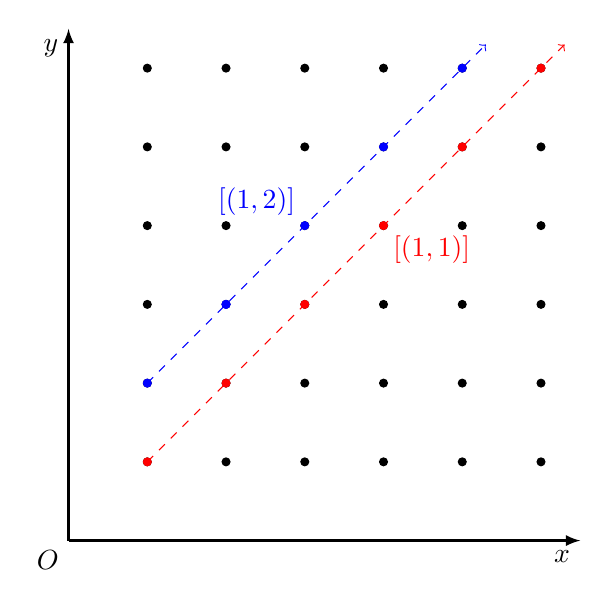
\begin{tikzpicture}[scale=1, transform shape]
                        \draw[latex-, thick] (0, 6.5) node[below left]{$y$} -- (0, 0);
                        \draw[latex-, thick] (6.5, 0) node[below left]{$x$} -- (0, 0);
                        \node[below left] at (0, 0){$O$};
                        \foreach \x in {1,...,6}{
                                \foreach \y in {1,...,6} {
                                        \draw[fill] (\x, \y) circle (0.05);
                                }
                        }
                        
                        \draw[color=red, dashed, ->] (1, 1) -- (6.3, 6.3);
                        \node[below right, color=red] at (4, 4){$[(1, 1)]$};
                        \foreach \x in {1,...,6} {
                                \draw[fill, color=red] (\x, \x) circle (0.05);
                        }
                        
                        \draw[color=blue, dashed, ->] (1, 2) -- (5.3, 6.3);
                        \node[above left, color=blue] at (3, 4){$[(1, 2)]$};
                        \draw[fill, color=blue] (1, 2) circle (0.05);
                        \draw[fill, color=blue] (2, 3) circle (0.05);
                        \draw[fill, color=blue] (2, 3) circle (0.05);
                        \draw[fill, color=blue] (3, 4) circle (0.05);
                        \draw[fill, color=blue] (4, 5) circle (0.05);
                        \draw[fill, color=blue] (5, 6) circle (0.05);
                \end{tikzpicture}
                \end{center}
        \end{enumerate}
        \clearpage

        \textbf{Solution 4.}\\
        Let $R$ be a relation on $\mathbb{R}^2\setminus\{(0,0)\}$ such that
        \[(x_1, x_2)\,R\,(y_1, y_2) \quad\text{if}\quad (y_1, y_2) = \alpha(x_1, x_2), \quad\alpha\neq 0\]
        \begin{enumerate}
                \item Let $x_i \in \mathbb{R}\setminus\{0\}$.
                Clearly, $R$ is reflexive since $(x_1, x_2) = (1)\cdot (x_1, x_2)$.

                Note that $\frac{1}{\alpha} \in \mathbb{R}\setminus\{0\}$, so if $(x_1, x_2)\,R\,(x_3, x_4)$, we have
                $(x_3, x_4)=\alpha(x_1, x_2) \Rightarrow (x_1, x_2) = \frac{1}{\alpha}(x_3, x_4)$. Therefore, $R$ is symmetric.
                
                If $(x_3, x_4) = \alpha(x_1, x_2)$ and $(x_5, x_6) = \beta(x_3, x_4)$, we have $(x_5, x_6) = (\alpha\beta)\cdot (x_1, x_2)$.
                Therefore, $R$ is transitive.

                Hence, $R$ is an equivalence relation.\qed
                
                \item For $(r, s) \in \mathbb{R}\setminus(0,0)$, we have
                \begin{align*}
                        [(r, s)] \;&=\; \{(x, y) \in \mathbb{R}^2\setminus\{(0, 0)\} : (r, s)\,R\,(x, y)\} \\
                                \;&=\; \{(x, y) \in \mathbb{R}^2\setminus\{(0, 0)\} : (x, y) = \alpha(r, s), \alpha \neq 0\} \\
                                \;&=\; \{(\alpha r, \alpha s) : \alpha, r, s \in \mathbb{R}\setminus\{0\}\}
                \end{align*}
                Clearly, each equivalence class $[(r, s)]$ is a line of slope $s/r$, through $(1, s/r)$, excluding the origin in the
                Cartesian plane.\\

                \begin{center}
                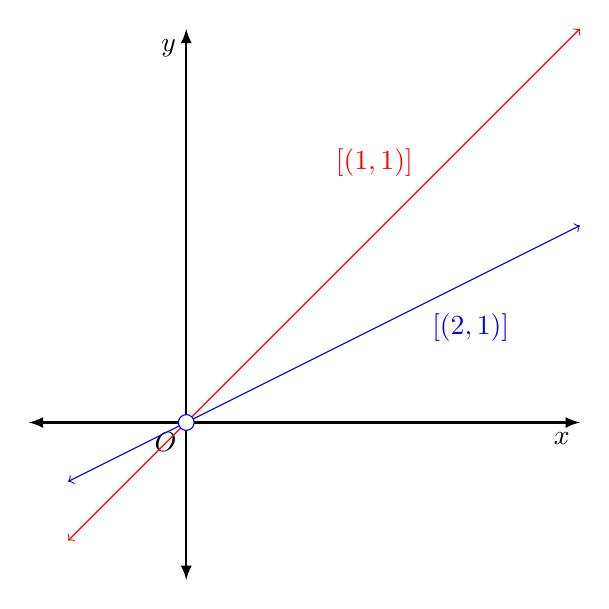
\begin{tikzpicture}[scale=1, transform shape]
                        \draw[latex-latex, thick] (0, 5) node[below left]{$y$} -- (0, -2);
                        \draw[latex-latex, thick] (5, 0) node[below left]{$x$} -- (-2, 0);
                        \node[below left] at (0, 0){$O$};
                        \node[above left, color=red] at (3, 3){$[(1, 1)]$};
                        \draw[<->, color=red] (-1.5, -1.5) -- (5, 5);
                        \node[below right, color=blue] at (3, 1.5){$[(2, 1)]$};
                        \draw[<->, color=blue] (-1.5, -0.75) -- (5, 2.5);
                        \draw[color=blue, fill=white] (0, 0) circle (0.1);
                \end{tikzpicture}
                \end{center}
 
        \end{enumerate}

        \textbf{Solution 5.}\\
        Let $n \in \mathbb{N}$ and $X$ be a set of $n$ elements.
        An arbitrary relation $R$ on $X$ is a subset of the Cartesian product $X\times X = X^2$.
        Note that for $(a, b) \in X^2$, $a$ can be any of the $n$ elements in $X$, and $b$ can be independently any
        of the $n$ elements in $X$. Thus, we have a total of $n^2$ elements in $X^2$.
        \begin{enumerate}
                \item Since $R$ is any subset $R \subseteq X^2$, we can say that a relation on $X$ is any $R \in \mathcal{P}(X^2)$.
                Thus, the total number of possible relations $R$ is the number of elements in $\mathcal{P}(X^2)$, i.e., $2^{n^2}$.

                \item Let $D = \{(x, x) : x \in X\}$ be the set of the diagonal elements of $X^2$. Clearly, there are $n$ elements in $D$.
                A reflexive relation $R$ must have $D \subseteq R$. Thus, of the $n^2$ elements of $X^2$, the $n$ diagonal elements
                are fixed -- the remaining $n^2 - n$ elements can be chosen to be or not to be in $R$, giving us a total of
                $2^{n^2 - n}$ such relations.

                \item Since $xRy \Rightarrow yRx$ if $x = y$, each of the $n$ diagonal elements of $X^2$ may or may not be present in a
                symmetric relation $R$ on $X$. Also, the presence of $(x, y) \in X^2\setminus D$ in $R$ forces the presence
                of $(y, x)$ in $R$. Thus, we have $(n^2 - n)/2$ choices for the non-diagonal elements, giving a total of
                $2^n \cdot 2^{(n^2 - n)/2} = 2^{(n^2 + n)/2}$ such relations.

                \item As before, we have $(n^2 - n)/2$ choices for non-diagonal elements to fulfil symmetry. The remaining diagonal
                elements are fixed to fulfil reflexivity, giving a total of $2^{(n^2 - n)/2}$ such relations.
        \end{enumerate}

\end{document}
